\section{Background}
\label{sec:background}
This section gives a brief overview of the theoretical considerations and concepts related to Monte-Carlo Tree Search. These ideas will be extended in Section \ref{sec:variations} and Section \ref{sec:use_cases}.
\begin{comment}
\subsection{Decision Trees}
\label{ss:decision_trees}
Two examples from \cite{fu2018monte}.
\paragraph{Example: Lottery}
\begin{figure}
    \centering
    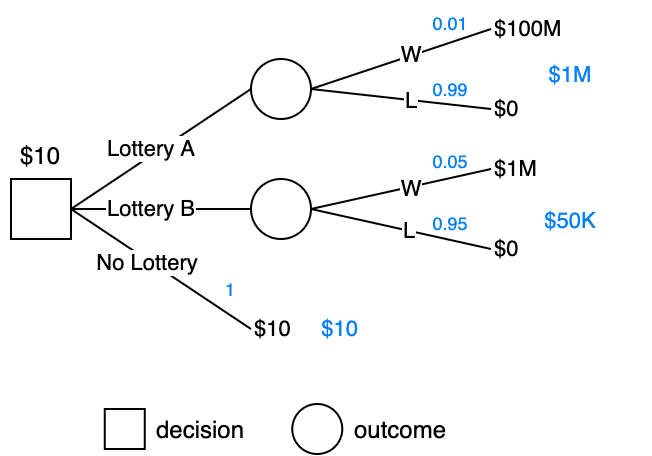
\includegraphics[width=0.6\textwidth]{img/lottery.png}
    \caption{A simple decision tree.}
    \label{fig:lottery}
\end{figure}
Figure \ref{fig:lottery} displays the simplest kind of decision tree: a single-step perfect information lottery. Picking the best decision is easily done by computing the expected value (displayed in blue) and selecting the maximum value. However, if the goal is not simply to maximize the reward without constraints but, e.g. to maximize the reward while ensuring that the actual reward is never zero the only possible decision is not to play any lottery. Constraints of this kind are modelled as so-called policies and are discussed in the following section.
\paragraph{Example: Tic-Tac-Toe}
At any point in time (i.e. at any \textit{state} of the game) there is only a limited number of moves available to the player and thus only a limited number of possible states \todo{Example}
There are three main kinds of decision trees in real-world games:
\begin{enumerate}[label=\arabic*)]
    \item \textit{Minimax}: This is the default strategy for two-player games. It selects the action that minimizes the opponent's maximum reward. Minimax can be generalized to both non-zero-sum games and for games with more than two players. 
    \item \textit{Expectimax}: In games where the transition function is probabilistic the Minimax-approach requires a weighted calculation of the rewards. This is called \textit{Expectimax}.
    \item \textit{Miximax}: Applying an approach similar to Expectimax to single-player games with imperfect information results in \textit{Miximax}.
\end{enumerate}
\end{comment}
\subsection{Game Theory}
\label{ss:game_theory}
According to \cite{browne2012survey} a game can be formally modelled as follows:
\begin{itemize}[noitemsep]
    \item $n \in \mathbb{N}$ players $k_1, \ldots, k_n$
    \item A set of states $S$ with an initial state $s_0$ and terminal states $S_T \subseteq S$
    \item A set of possible actions $A$
    \item A state transition function $f: S \times A \to S$
    \item A reward function $r: S \to \mathbb{R}^k$
\end{itemize}
A game starts in state $s_0$ and progresses according to the state transition function $f$ which at point $t$ gives us the next state $s_{t+1}$ defined by the action $a$ taken by a player $k_i$. Usually it is only one players's turn at any given point $t$. The reward function $r$ determines points gained or lost by players through these actions. The game ends when a terminal state $s_j \in S_T$ is reached. The probability of a given player choosing any action $a$ is determined by its \textit{policy}. Games can be classified using the following criteria:
\begin{enumerate}[label=\alph*)]
    \item \textit{zero sum}: Do the rewards given to all players add up to zero?
    \item \textit{information}: Is the complete state of the game known to the players?
    \item \textit{determinism}: Does change play a part?
    \item \textit{sequential}: Can multiple players choose an action simultaneously?
    \item \textit{discreteness}: Are actions atomic or do they take time? 
\end{enumerate}
An important category of games are so-called \textit{combinatorial games}. They are zero-sum, perfect information, deterministic, sequential and discrete. Examples are \textit{Go}, \textit{Chess} and \textit{Tic-Tac-Toe}.

\subsection{Monte Carlo Methods and Multi Armed Bandits}
The basic idea of Monte-Carlo based methods is that of \textit{sampling}. While operating on a very large domain it is not feasible to simply do calculations which consider all possible elements of said domain. We therefore have to select only a (usually much smaller) subset of these elements. In the following we will apply this idea to game theory. 
\todo{explain}
The so-called Q-value of an action is defined as the expected reward of this action:
\begin{equation}
    Q(s,a)= \frac{1}{N(s,a)} \sum_{i=1}^{N(s)} \mathbb{I}_i(s,a)z_i
\end{equation}

In the \textit{Multi-Armed-Bandit} problem a player has to choose one of $K$ arms out of the set $\mathcal{K} = \{1,\ldots,K \}$ at each one of $T$ rounds. Sometimes the number of rounds $T$ is called the \textit{horizon} of the game and the decision points $t_1,\ldots,t_T$ are called the decision epochs. Each arm has a value associated with it. These rewards $X^k_t$ of arm $k$ at decision epoch $t$ can be modelled as a random variable with values $X_k^t \in [0,1]$ and expected value $\mu_t^k = \mathbb{E}[X^k_t]$. The best possible reward is therefore given via 
\begin{equation*}
\mu^\star_t = \max_{k \in \mathcal{K}} \{ \mu^k_t\}    
\end{equation*}
In the \textit{non-stationary} problem formulation the value of each arm may change over the course of the game. The extent of this change is called \textit{temporal variation} and (according to \cite{besbes2019optimal}) is measured by the following metric for $T > 1$:
\begin{equation}
    \mathcal{V}(\mu;T) \coloneqq \sum_{t=1}^{T-1} \sup_{k \in \mathcal{K}} \left| \mu_t^k - \mu_{t+1}^k \right|
\end{equation}
The performance of a given policy can be measured relative to an oracle which has perfect information and picks the best possible choice. The difference in rewards between the policy and the oracle is called \textit{regret}. After n epochs it is given as:
\todo{notation inconsistent}
\todo{lower bound for static case}
\begin{equation}
    R_N = \mu^\star n - \mu_i \sum_{j=1}^K \mathbb{E}[T_j(n)]
\end{equation}

Any policy aims to minimize this value. As shown in \cite{lai1985asymptotically} there exist no policy with a growth of the regret slower than $O(\ln n)$ for most reward distributions (i.e., distributions of the rewards $X^k_t$).


For \textit{bandit problems} (see e.g. \cite{lattimore2018bandit} for an introduction) it is desirable to know the \textit{Upper Confidence Bound} (UCB) that any given arm will be optimal in the game-theoretic sense described in Section \ref{ss:game_theory}. In the formulation of \cite{sironi2019comparing} it is given by:
\begin{equation}
    \text{UCB1} = \underbrace{Q(s,a)}_{(\ast)} +  \underbrace{\sqrt{\frac{2 \ln N(s)}{N(s,a)}}}_{(\ast \ast)}
\end{equation}
$N(s)$ is the the number of times state $s$ has been visited, and $N(s,a)$ denotes how often action $a$ has been selected when $s$ has been visited.
Since this term is maximized by any reasonable policy (i.e. one that aims to win) its parts can be analyzed quite easily: The first term $(\ast)$ facilitates the exploration of higher reward choices while the second term $(\ast \ast)$ does the same for less-visited, currently deemed less promising choices. This UCB1-sampling strategy is most prominently used in the UCT-MCTS variant described below. 
\subsection{Monte Carlo Tree Search}
The so-called game tree contains all possible states a game could be in. Its nodes represent the states and its edges $(s_i,s_j)$ represent the action leading from state $s_i$ to state $s_j$. Thus it is generally not possible to completely search the tree because the number of nodes is too large. Monte Carlo Tree Search is an algorithm for traversing game trees utilizing the idea of sampling. The search tree consists of nodes representing (possible) states of the game while their links describe actions that lead from one state to the other. MCTS iteratively builds a search tree while a certain condition holds, usually referred to as the computational budget. The algorithm consists of four basic steps:
\begin{enumerate}[label=\arabic*)]
    \item \textit{Selection}: Beginning from the root node the tree is traversed using a child selection policy until an expandable node is reached: that is, a node representing a non-terminal state that has unvisited children.
    \item \textit{Expansion}: One or more child nodes are added to the tree if the actions leading to them are possible.
    \item \textit{Simulation}: From the state of the new node a simulation of the game is run according to the \textit{Default Policy}. Its results are taken to be the value of the node.
    \item \textit{Backpropagation}: The new values are backed up through the tree which may result in updates to the statistics of the nodes.
\end{enumerate}
\begin{figure}[htbp]
    \centering
    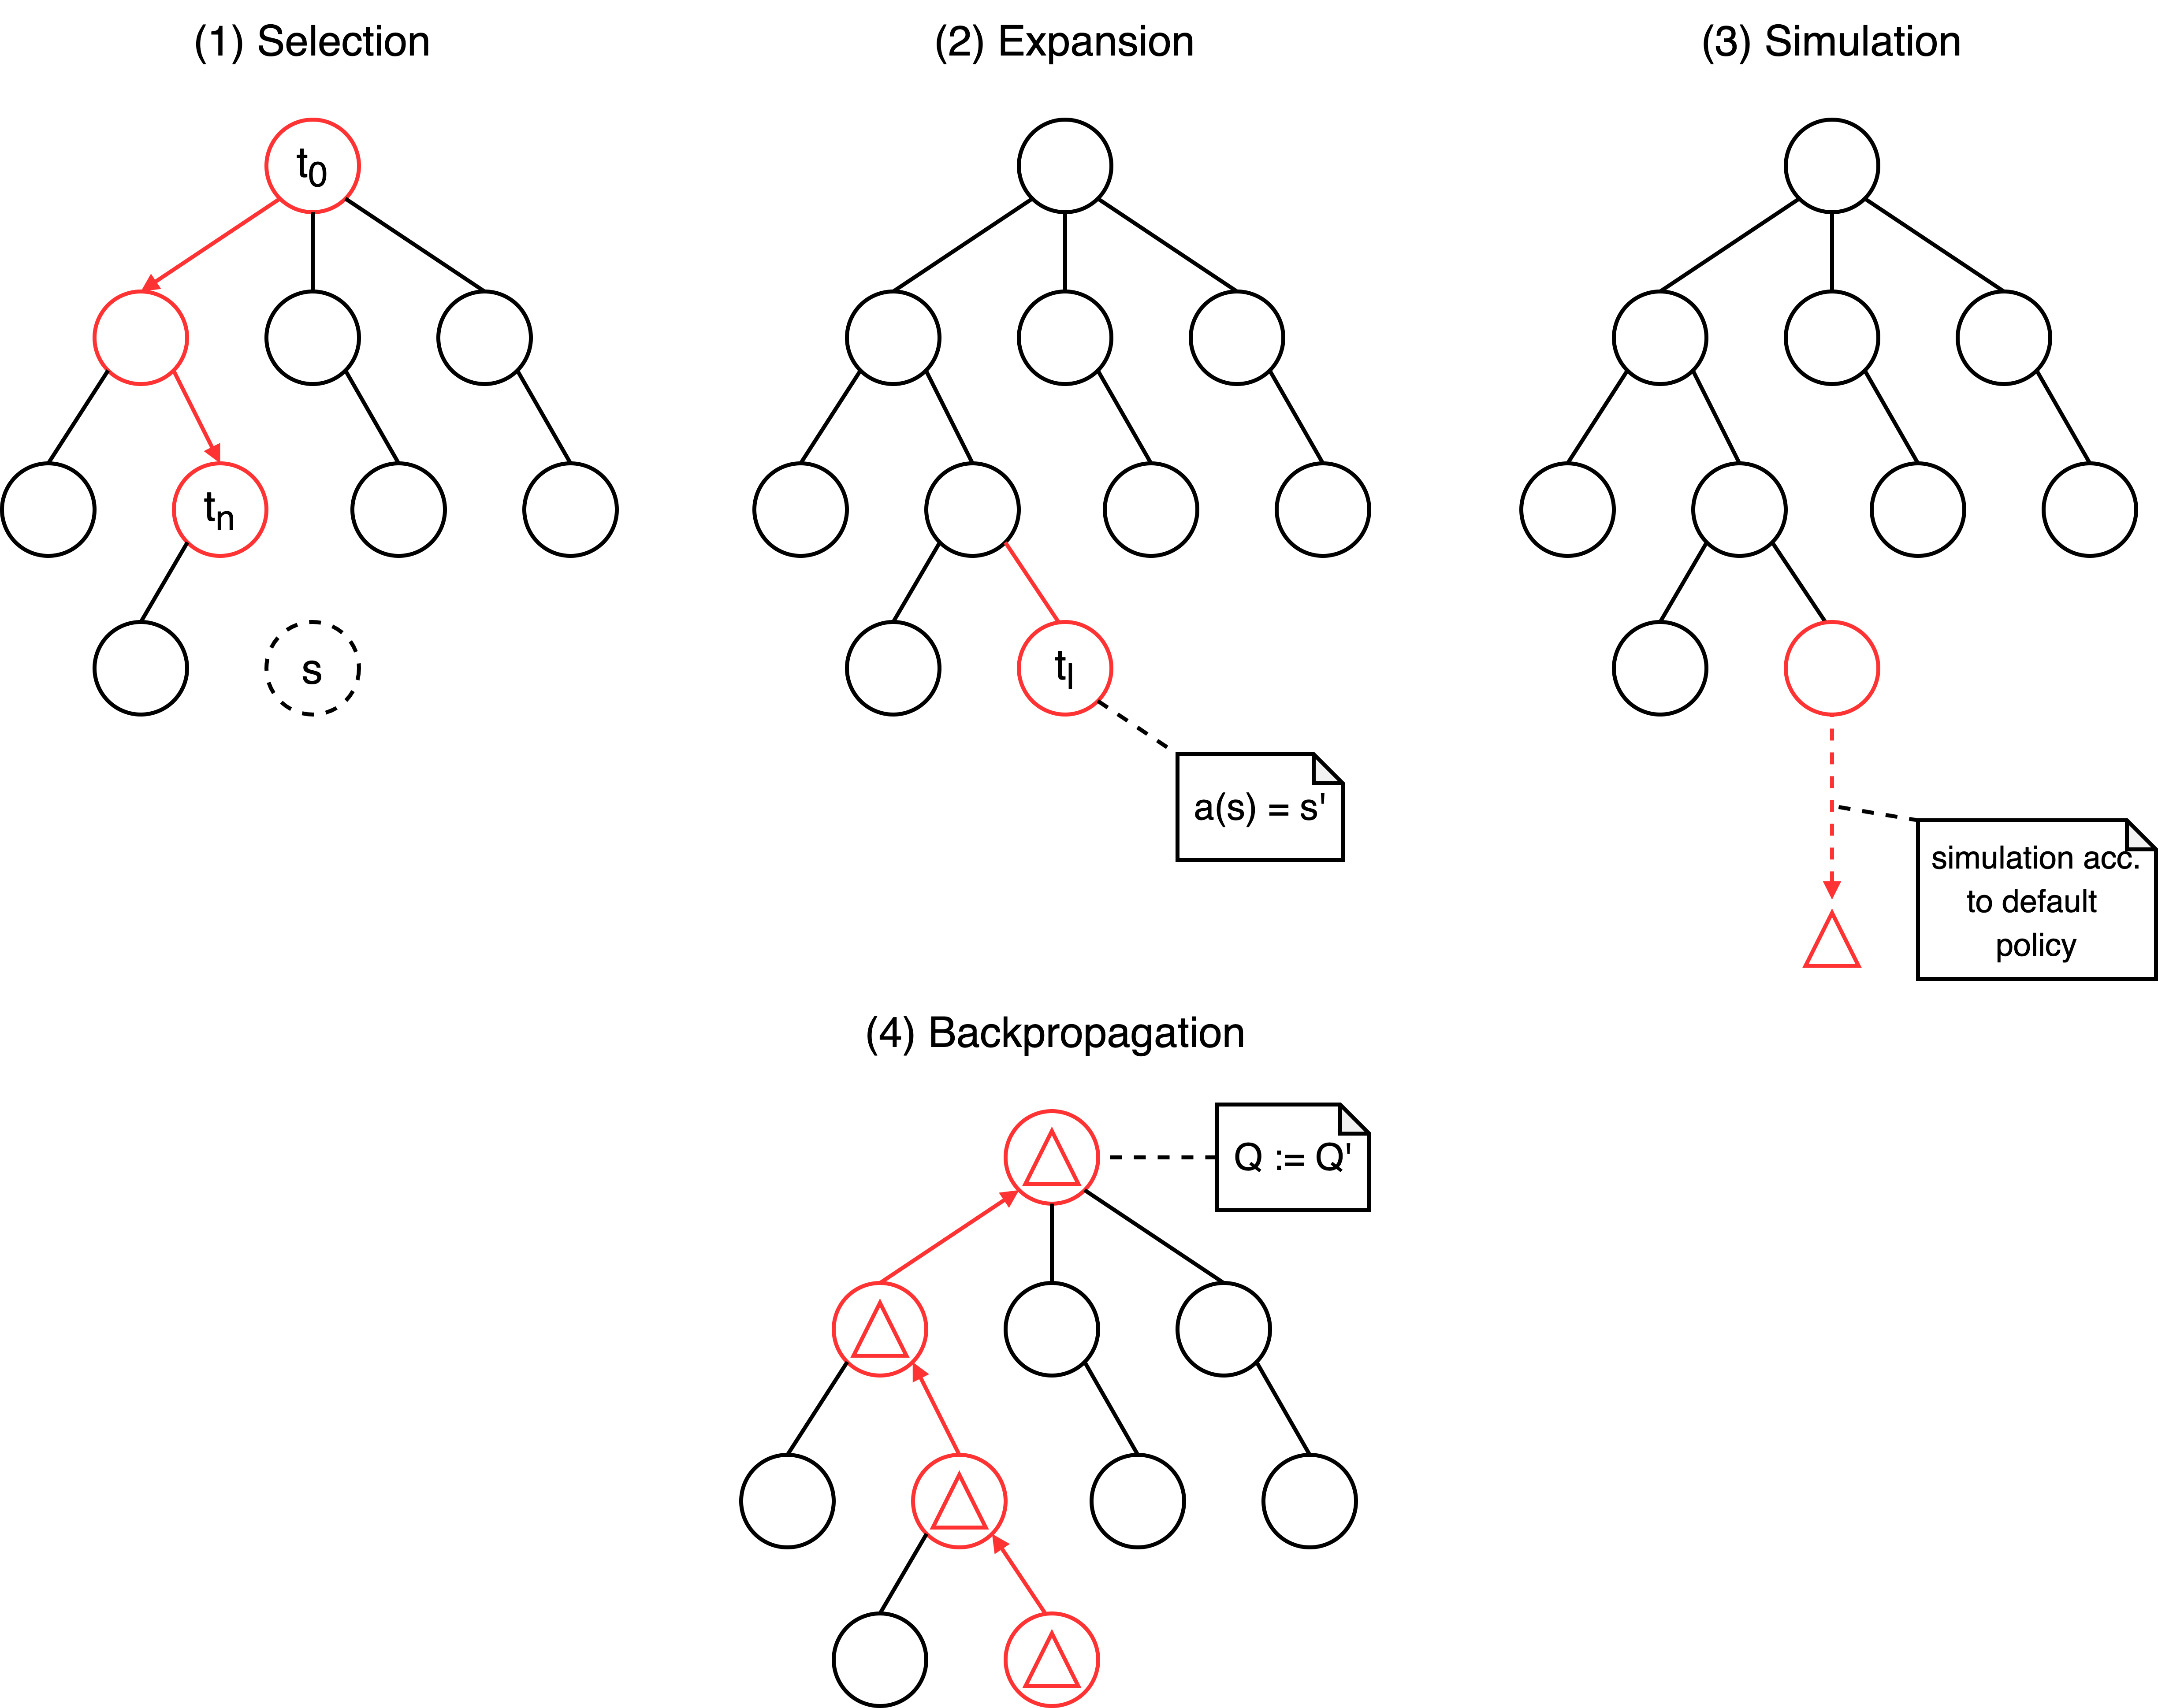
\includegraphics[width=0.8\textwidth]{img/mcts-basics.png}
    \caption{The four basic MCTS steps}
    \label{fig:mcts_basics}
\end{figure}
\begin{algorithm}[htbp]
\begin{algorithmic}
\Function{MCTS}{$s_0$} 
    \State create root node $v_0$ with state $s_0$
    \While{within computational budget}
    \State $v_l \gets$ \Call{TreePolicy}{$v_0$} \Comment{$v_l$ is the last node reached}
    \State $\Delta \gets$ \Call{DefaultPolicy}{$s(v_l)$} \Comment{simulate from state node $v_l$ with state $s_l$}
    \State \Call{Backup}{$v_l,\Delta$}
    \EndWhile
    \State \Return \Call{$a$}{\Call{bestChild}{$v_0$}$)$} \Comment{return most valuable action $a$}
\EndFunction
\end{algorithmic}
\caption{Basic Monte Carlo Tree Search function.}
\label{alg:mcts_basic}
\end{algorithm}
\cite{browne2012survey} identifies the following three characteristics of Monte Carlo Tree Search:
\begin{enumerate}[label=\alph*)]
    \item \textit{Aheuristic}: There is no concrete domain knowledge required. MCTS can be applied to any domain that can be modelled as a tree. However, any available knowledge can greatly improve the performance of the search. Whether this manifests in modelling design decision of the problem itself or heuristics for use in the tree and/or simulation policy.   
    \item \textit{Anytime}: Due to the immediate backpropagation of each game outcome the values of all nodes are always up-to-date. This makes it possible to return (i.e., end the search and return the root action) at any time.
    \item \textit{Asymmetric}: Since more promising nodes are favoured by the search the tree does not grow at the same rate (of iterations) everywhere. The tree can gain an irregular, asymmetric shape.
\end{enumerate}
\subsection{UCT}
\label{ss:uct}
UCT (Upper Confidence Bound for Trees) is an important family of MCTS-Algorithms. They follow the basic MCTS-schema shown in \ref{alg:mcts_basic} but define their own default- and tree-policies. In the following we discuss an implementation of UCT in pseudocode for games (except for some nomenclature UCT is of course applicable to all generic search problems). All possible states of the game are described using nodes, each node $v$ has four members:
\begin{itemize}
    \item associated state $s(v)$
    \item incoming action $a(v)$
    \item total simulation reward $Q(v)$
    \item visit count $N(v)$
\end{itemize} Initially all nodes except the initial state of the game are not part of the search tree but can be added (\enquote{chosen}) during the search. More precisely: While the budget is not exhausted a child node is selected according to the tree policy, which is discussed in detail below. Then the simulation is executed according to the default policy of choosing actions (and thus child nodes) uniformly at random. When a terminal state is reached the results are backpropagated, i.e. updating the four entries in the nodes. When the budget is used up the best node is returned as a result.

A key concept of UCT is the treatment of child-node selection as a MAB-problem. With this abstraction we can use the UCB1 equation from above in the tree policy (cf. Algorithm \ref{alg:uct_tree_policy}):
\begin{equation}
    UCT(v) = \frac{Q(v')}{N(v')}+C_p \cdot \sqrt{\frac{2 \ln N(v)}{N(v')}}
\end{equation} where $v'$ are children of $v$. There are two differences to default UCB1. One is the treatment of $a$ and $s$ as nodes to fit the pseudocode. In the next sections however we omit the treatment of $a(v)$ and $s(v)$ as members of a node for convenience and just write $a$ and $s$. Read \enquote{state $s$ represented by a node} and \enquote{action $a$ which leads to the state $s$ represented by a node}. More consequential however is the parameter $C_p > 0$ that mediates between exploration and exploitation. Usually we just set $C_p = \frac{1}{2} $ but this can of course be tuned. 

Now the child selection just translates to maximizing this function. UCT always chooses the child node $v^\star$ (or, more precisely, the action $a^\star$ leading to $v^\star$) with
\begin{equation*}
    v^\star = \underset{v' \in v.children}{\arg \max} UCT(v)
\end{equation*}  
\begin{algorithm}[htbp]
\begin{algorithmic}
\Function{TreePolicy}{$v$} 
    \While{$v$ is nonterminal}
    \If{v is not fully expanded}
    \State \Return{\Call{Expand}{$v$}}
    \Else
    \State $v \gets$ \Call{BestChild}{$v,C_p$}
    \EndIf
    \EndWhile
    \Return{$v$}
\EndFunction \\
\Function{Expand}{$v$}
\State choose untried $a \in A(s(v))$
\State add new child $v'$ to $v.children$ with $s(v') = f(s(v),a)$ and $a(v') = a$
\State \Return{$v'$}
\EndFunction \\
\Function{BestChild}{$v,c$}
\State \Return{$\underset{v' \in v.children}{\arg \max} \frac{Q(v')}{N(v')}+c \cdot \sqrt{\frac{2 \ln N(v)}{N(v')}}$}
\EndFunction
\end{algorithmic}
\caption{The tree policy of UCT.}
\label{alg:uct_tree_policy}
\end{algorithm}
\begin{algorithm}[htbp]
\begin{algorithmic}
\Function{DefaultPolicy}{$s$}
\While{$s$ is non-terminal}
\State choose $a \in A(s)$ uniformly at random
\State $s \gets f(s,a)$
\EndWhile
\State \Return{reward for $s$}
\EndFunction \\

\Function{Backup}{$v, \Delta$} \Comment{no strictly speaking part of the default policy}
\While{$v$ is not null}
\State $N(v) \gets N(v) + 1$
\State $Q(v) \gets Q(v) + \Delta(v,p)$
\State $v \gets v.parent$
\EndWhile
\State $N(v) \gets N(v) + 1$
\State $Q(v) \gets Q(v) + \Delta$
\State $\Delta \gets - \Delta$
\State $v \gets v.parent$
\EndFunction
\end{algorithmic}
\caption{The default policy of UCT.}
\label{alg:uct_default_policy}
\end{algorithm}


\subsection{Heuristics and RAVE}
There exist many heuristics for MCTS. That is use-case specific enhancements and modifications of the basic MCTS steps (most importantly tree and default policy). In the context of MAB and UCT child selection one important heuristic is \textit{All Moves As First} (\textit{AMAF}) and its enhancement \textit{Rapid Action Value Estimation} (\textit{RAVE}). AMAF treats every action used during the simulation (i.e. chosen by the default policy) as if it was chosen by the tree policy. This is illustrated in Figure \ref{fig:amaf} in the context of Tic-Tac-Toe. Beginning from the given state UCT selects $(C,2)$ as the next black position and $(A,1)$ for the next white one. Then the progress of the game is simulated with $(B,1)$ black, $(A,3)$ white and $(C,3)$ black, leading to the terminal state displayed and resulting in a win for black. During the backpropagation the values for the nodes visited by UCT are updated as before. But due to AMAF more nodes are updated: Since $(B,1)$ (as well as the others) could have been chosen by UCT and was used during the simulation its statistics are updated as well. The value generated this way is called \textit{AMAF score} and is generally separate from the UCT value.
\begin{figure}
    \centering
    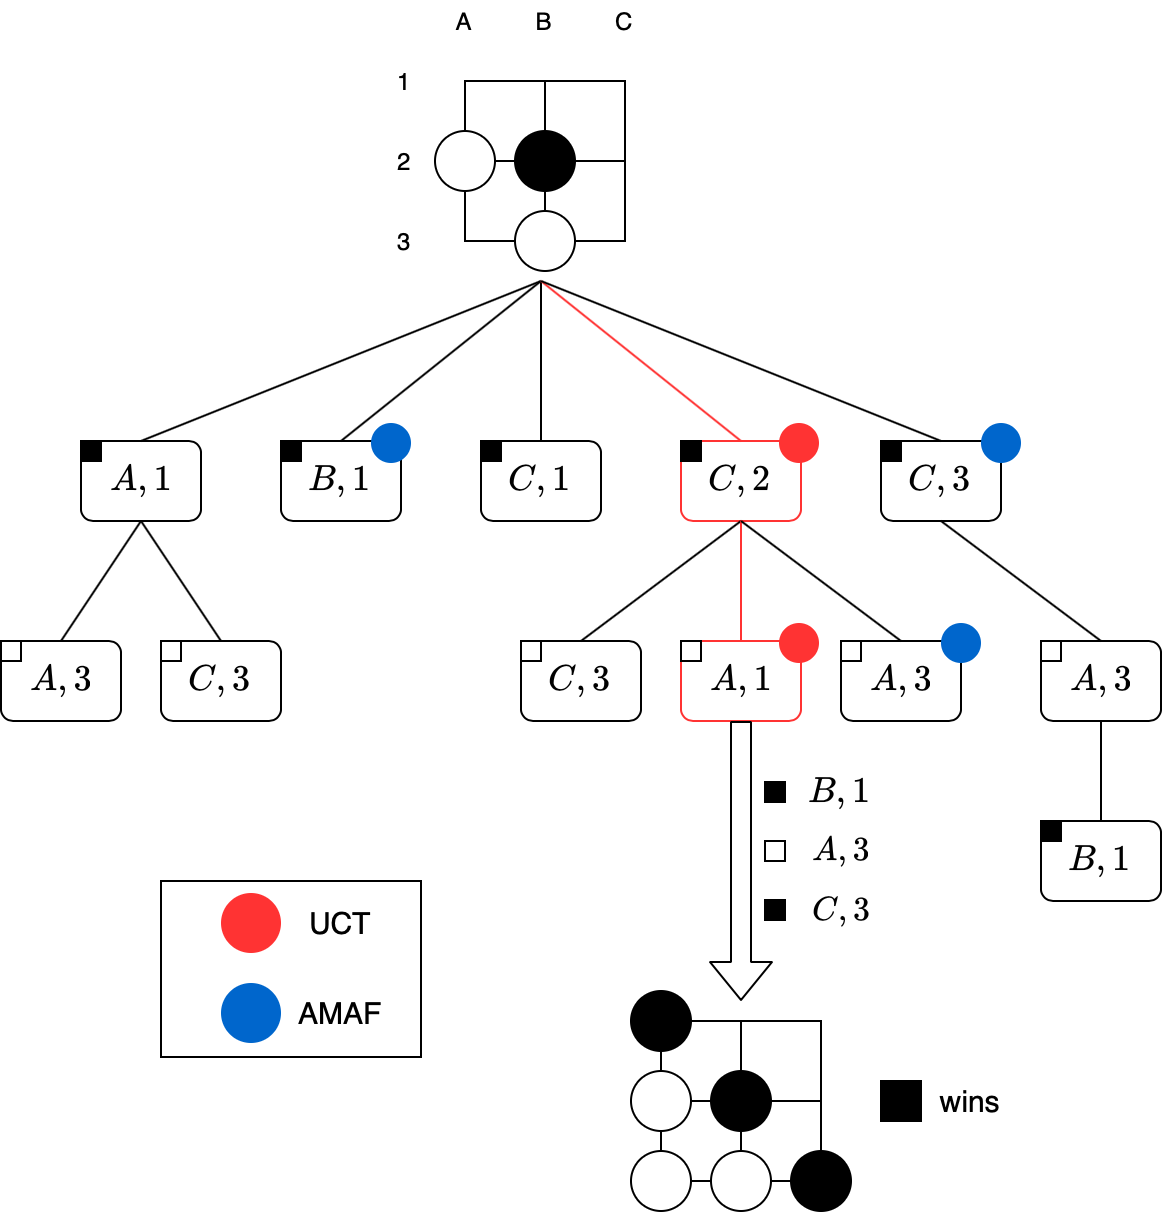
\includegraphics[width=0.7\textwidth]{img/amaf.png}
    \caption{The AMAF-heuristic updates all nodes that are used in the simulation as if they were selected by UCT directly.}
    \label{fig:amaf}
\end{figure}
\textit{RAVE} is a way of combining the UCT value $Q(\cdot)$ and AMAF score $AMAF(\cdot)$ for an action $a$ at a state $s$ via the equation:
\begin{equation}
    \beta(s) \cdot Q(s,a) + (1 - \beta(s)) \cdot AMAF(s',a)
    \label{eq:rave}
\end{equation}
where 
\begin{equation*}
    \beta(s) = \sqrt{\frac{K}{3 \cdot N(s) + K}}
\end{equation*}
$N(s)$ denotes the number of visits to state $s$. The term $AMAF(s',a)$ is the average result of all simulations (i.e. the backpropagated value $\Delta$) in which $a$ was selected after $s'$ was visited. $s'$ is an ancestor of $s$. Which ancestor is dependent on the actual formulation, in its basic form \textit{RAVE} always selects the direct predecessor of $s'$ on the path through the search tree. \textit{GRAVE}, described in Section \ref{sec:variations} modifies this selection procedure. $K$ is the so-called \textit{equivalence parameter} which determines the number of simulations where UCT and AMAF are both considered with equal weight.